\documentclass[12pt]{article}
\usepackage[T1]{fontenc}
\usepackage[T1]{polski}
\usepackage[utf8]{inputenc}
\newcommand{\BibTeX}{{\sc Bib}\TeX}
\usepackage{graphicx}
\usepackage{amsfonts}
\usepackage{amsmath}
\usepackage{listings}

\setlength{\textheight}{21cm}
\setlength{\emergencystretch}{3em}

\lstset{basicstyle=\ttfamily\footnotesize, columns=fullflexible, frame=lines,
        showstringspaces=false, breaklines=true}

\title{{\bf Zadanie nr 4 - Sieć samoorganizująca się SOM w~kompresji obrazów}\linebreak
Inteligentna Analiza Danych}
\author{Jędrzej Kostyk 264339}
\date{2 listopada 2026}

\begin{document}
\clearpage\maketitle
\thispagestyle{empty}
\newpage
\setcounter{page}{1}
\section{Cel zadania}

Celem zadania było zaimplementowanie jednowarstwowej liniowej sieci samoorganizującej się (SOM),
trenowanej bez nadzoru ze współzawodnictwem neuronów, i~użycie jej do kompresji obrazów
w~skali szarości. Dla ramki $2\times2$ piksele dobrano parametry nauki, a~następnie zbadano,
jak początkowa liczba neuronów ($4$--$256$) wpływa na współczynnik kompresji CR i~jakość obrazu
odtworzonego PSNR, oraz wykreślono zależność CR od PSNR. Dodatkowo sprawdzono wpływ rozmiaru
ramki i~sposobu inicjalizacji wag.

\section{Wstęp teoretyczny}

\textbf{Sieć SOM i~trening ze współzawodnictwem.} Sieć ma architekturę taką jak MADALINE: jedną
warstwę $K$ neuronów liniowych, które liczą iloczyny skalarne $y_i=\mathbf{w}_i\cdot\mathbf{x}$
znormalizowanego wejścia ze swoimi znormalizowanymi wagami~\cite{wyklad3,kohonen1990}. Wzorce
treningowe zawierają tylko wejścia (uczenie nienadzorowane). Po podaniu wzorca wybierany jest
neuron zwycięski $m=\arg\max_i y_i$ i~tylko jego wagi są modyfikowane według reguły
,,zwycięzca bierze wszystko'' (WTA, Algorytm~2.1 w~\cite{wyklad3}):
\begin{equation}
 \mathbf{w}_m \leftarrow \frac{\mathbf{w}_m+\eta\,(\mathbf{x}-\mathbf{w}_m)}{\|\mathbf{w}_m+\eta\,(\mathbf{x}-\mathbf{w}_m)\|} .
 \label{eq_som}
\end{equation}
Wagi zwycięzcy przesuwają się w~stronę wzorca, więc po treningu każdy żywy neuron reprezentuje
,,średni'' kierunek jednego skupiska wektorów wejściowych. Neurony, które nigdy nie wygrały,
nazywa się \emph{martwymi} i~usuwa się je z~sieci.

\textbf{Kompresja obrazu (Algorytm~2.2 w~\cite{wyklad3}).} Obraz $N\times N$ dzieli się na
$(N/n)^2$ ramek $n\times n$, które po spłaszczeniu i~normalizacji są wzorcami treningowymi.
Po treningu i~usunięciu martwych neuronów każda ramka $\mathbf{x}_k$ jest kodowana dwiema liczbami
całkowitymi: indeksem neuronu zwycięskiego $\mathcal{L}_k$ (kierunek, czyli ,,kształt'' ramki) oraz
skwantowaną długością $\mathcal{T}_k=\mathrm{round}(\|\mathbf{x}_k\|/q)$ (jasność ramki), gdzie $q$ to
współczynnik kwantyzacji. Do pliku trafiają też wagi wszystkich $K$ żywych neuronów $\mathcal{W}$.
Dekodowanie odtwarza ramkę jako $\mathbf{x}'_k=q\,\mathcal{T}_k\,\mathcal{W}_{\mathcal{L}_k}$. Jest to
w~istocie kwantyzacja wektorowa~\cite{gray1984}: zamiast pikseli zapamiętuje się numer ,,wzorcowej''
ramki ze słownika.

\textbf{Miary efektywności.} Jakość obrazu odtworzonego mierzy szczytowy stosunek sygnału do szumu
\begin{equation}
 \mathrm{PSNR}=10\log_{10}\frac{255^2}{\mathrm{MSE}}\ \mathrm{[dB]},\qquad
 \mathrm{MSE}=\frac{1}{N^2}\sum_{i,j}(x_{ij}-x'_{ij})^2 ,
 \label{eq_psnr}
\end{equation}
a~stopień kompresji to iloraz liczby bitów obrazu oryginalnego i~skompresowanego (wzór 2.4
w~\cite{wyklad3}):
\begin{equation}
 \mathrm{CR}=\frac{8N^2}{N_{\mathcal{W}}+N_{\mathcal{L}}+N_{\mathcal{T}}},
 \label{eq_cr}
\end{equation}
\begin{align*}
 N_{\mathcal{W}}&=8Kn^2, &
 N_{\mathcal{L}}&=\Big(\frac{N}{n}\Big)^2\big(\lfloor\log_2(K-1)\rfloor+1\big),\\
 & &
 N_{\mathcal{T}}&=\Big(\frac{N}{n}\Big)^2\big(\lfloor\log_2\max_k\mathcal{T}_k\rfloor+1\big).
\end{align*}
Składniki mianownika to liczby bitów potrzebne na wagi (8 bitów na wagę), indeksy neuronów
zwycięskich i~skwantowane długości ramek.

\textbf{Ograniczenie CR dla ramki $2\times2$.} Ramka oryginalna zajmuje $8\cdot4=32$ bity. Po kompresji
potrzeba co najmniej 1 bitu na indeks, a~przy $q=10$ największa długość ramki ($2\cdot255=510$) daje
$\mathcal{T}\le51$, czyli 6 bitów. Dlatego nawet przy jednym neuronie
$\mathrm{CR}\le32/7\approx4{,}57$. Każde podwojenie liczby żywych neuronów dokłada 1 bit na ramkę.

\textbf{Szczegóły implementacji.} Program \texttt{som.py} realizuje Algorytmy 2.1 i~2.2.
Wagi początkowe są losowane z~$[-1,1]$ i~normalizowane, a~kolejność ramek jest losowana w~każdej
epoce. Neuron jest uznawany za martwy, gdy jego wagi nie zostały zmienione ani razu. Wagi zapisane
w~,,pliku'' kwantujemy do 8 bitów, zgodnie z~założeniem wzoru~(\ref{eq_cr}), a~obraz odtworzony
zaokrąglamy do liczb całkowitych z~$[0,255]$. W~przykładowym raporcie w~materiałach do wykładu
użyto 5 bitów na wagę, a~nie 8 jak we wzorze~(\ref{eq_cr}). Liczba bitów na wagę jest więc parametrem
programu (\texttt{-{}-weight-bits}, domyślnie 8). Przy ramce $2\times2$ wagi stanowią tylko 1--2\%
rozmiaru pliku, więc wybór 5 albo 8 bitów zmienia CR o~mniej niż 1\%.

\section{Eksperymenty i wyniki}

Wspólne założenia wszystkich eksperymentów:
\begin{itemize}
 \item obrazy \texttt{zelda}, \texttt{cameraman} i~\texttt{peppers} z~materiałów do kursu,
       $128\times128$ pikseli, 8-bitowa skala szarości (dostarczone jako pliki PNG),
 \item ramka $2\times2$, czyli $4096$ ramek i~wektory o~4 elementach (o~ile nie podano inaczej),
 \item parametry domyślne: $20$ epok, $\eta=0{,}2$, $q=10$, 8 bitów na wagę,
 \item każdy wariant uruchomiono z~5 ziarnami generatora (różne wagi początkowe i~kolejność ramek),
       podano średnie, a~w~tabelach parametrów także odchylenia standardowe PSNR.
\end{itemize}

Przykładowy raport programu (\texttt{python som.py images/zelda.png -{}-neurons 64}):
\begin{lstlisting}
resolution             = 128 x 128
frame_size             = 2 x 2

num_frames             = 4096
num_neurons (start)    = 64
num_neurons            = 11
num_weights_per_neuron = 4
max_quantized_length   = 34

bits_per_index         = 4
bits_per_length        = 6
bits_per_weight        = 8

org_size_bits          = 131072
cmp_size_bits          = 41312

w_1  = [ 0.373   0.404   0.506   0.671]
w_2  = [ 0.420   0.537   0.467   0.561]
w_3  = [ 0.624   0.357   0.631   0.302]
w_4  = [ 0.741   0.420   0.388   0.349]
CR   = 3.173
PSNR = 31.789 dB
\end{lstlisting}

%%%%%%%%%%%%%%%%%%%%%%%%%%%%%%%%%%%%%%%%%%%%%%%%%%%%%%%%%%%%%%%%%%%%%%%%%%%%%%%%%%%%%%%%%%%%%%%%%%%%%%%%%%%%%%%%%
% PODROZDZIAŁ PT. EKSPERYMENT NR 1
%%%%%%%%%%%%%%%%%%%%%%%%%%%%%%%%%%%%%%%%%%%%%%%%%%%%%%%%%%%%%%%%%%%%%%%%%%%%%%%%%%%%%%%%%%%%%%%%%%%%%%%%%%%%%%%%%

\subsection{Eksperyment nr 1 -- dobór parametrów nauki}

\subsubsection{Założenia}

Obraz \texttt{zelda}, ramka $2\times2$, $K=64$ neurony. Zmieniano po jednym parametrze, a~pozostałe
miały wartości sugerowane w~specyfikacji.

\subsubsection{Przebieg}

Zbadano $\eta\in\{0{,}01;\dots;0{,}9\}$, liczbę epok od 1 do 50 oraz $q$ od 1 do 40. Dla każdej
wartości wykonano 5 treningów.

\subsubsection{Rezultat}

\begin{table}[h!]
 \caption{Wpływ parametrów nauki na PSNR i~CR (\texttt{zelda}, $K=64$, średnia z~5 uruchomień)}
 \centering
 \small
 \vspace{0.2cm}
 \begin{tabular}{c c c c}
  \hline\hline\\[-0.4cm]
  $\boldsymbol{\eta}$ & \textbf{PSNR [dB]} & \textbf{CR} & \textbf{żywe}\\[0.1cm]
  \hline
  $0{,}01$ & $31{,}05\pm0{,}37$ & $3{,}172$ & $11{,}4$ \\
  $0{,}05$ & $31{,}93\pm0{,}24$ & $3{,}168$ & $12{,}8$ \\
  $0{,}1$ & $32{,}27\pm0{,}13$ & $3{,}169$ & $12{,}6$ \\
  $0{,}2$ & $31{,}94\pm0{,}52$ & $3{,}167$ & $13{,}2$ \\
  $0{,}5$ & $31{,}14\pm0{,}74$ & $3{,}166$ & $13{,}6$ \\
  $0{,}9$ & $29{,}72\pm1{,}29$ & $3{,}166$ & $13{,}8$ \\
  \hline
 \end{tabular}\hspace{0.4cm}
 \begin{tabular}{c c c c}
  \hline\hline\\[-0.4cm]
  \textbf{epoki} & \textbf{PSNR [dB]} & \textbf{CR} & \textbf{żywe}\\[0.1cm]
  \hline
  $1$ & $30{,}62\pm0{,}35$ & $3{,}244$ & $10{,}4$ \\
  $2$ & $30{,}88\pm0{,}42$ & $3{,}171$ & $11{,}6$ \\
  $5$ & $31{,}77\pm0{,}24$ & $3{,}170$ & $12{,}2$ \\
  $10$ & $31{,}98\pm0{,}65$ & $3{,}168$ & $12{,}8$ \\
  $20$ & $31{,}94\pm0{,}52$ & $3{,}167$ & $13{,}2$ \\
  $50$ & $32{,}41\pm0{,}30$ & $3{,}167$ & $13{,}4$ \\
  \hline
 \end{tabular}

 \vspace{0.3cm}
 \begin{tabular}{c c c c}
  \hline\hline\\[-0.4cm]
  $\boldsymbol{q}$ & \textbf{PSNR [dB]} & \textbf{CR} & \textbf{żywe}\\[0.1cm]
  \hline
  $1$ & $32{,}17\pm0{,}55$ & $2{,}442$ & $13{,}2$ \\
  $2$ & $32{,}16\pm0{,}55$ & $2{,}644$ & $13{,}2$ \\
  $5$ & $32{,}12\pm0{,}54$ & $2{,}882$ & $13{,}2$ \\
  $10$ & $31{,}94\pm0{,}52$ & $3{,}167$ & $13{,}2$ \\
  $20$ & $31{,}33\pm0{,}45$ & $3{,}515$ & $13{,}2$ \\
  $40$ & $29{,}48\pm0{,}30$ & $3{,}949$ & $13{,}2$ \\
  \hline
 \end{tabular}
 \label{tab_param}
\end{table}

\noindent Wyniki są w~Tab.~\ref{tab_param}.
\begin{itemize}
 \item \textbf{Współczynnik uczenia:} wartości $0{,}05$--$0{,}2$ dają podobny PSNR (ok.\ 32~dB,
       różnice mniejsze niż rozrzut między uruchomieniami). Zbyt małe $\eta=0{,}01$ nie pozwala wagom
       dojść do środków skupisk w~20 epokach. Zbyt duże ($0{,}5$; $0{,}9$) obniża PSNR i~zwiększa rozrzut,
       bo wagi zwycięzcy ,,skaczą'' za każdą kolejną ramką zamiast uśredniać skupisko.
 \item \textbf{Liczba epok:} już po 5 epokach PSNR jest bliski wartości końcowej. Dalsze epoki dają
       ok.\ $0{,}5$~dB, więc sugerowane 20 epok jest wystarczające.
 \item \textbf{Współczynnik kwantyzacji $q$:} nie wpływa na trening, tylko na zapis jasności ramek.
       Większe $q$ to mniej bitów na długość ramki, czyli wyższe CR, ale też większy błąd jasności.
       Przy $q=40$ CR rośnie do $3{,}95$, a~PSNR spada o~$2{,}5$~dB. Przy $q\le10$ PSNR prawie się
       nie zmienia, bo błąd jest wtedy zdominowany przez kwantyzację kształtu ramek przez sieć.
\end{itemize}
Do dalszych eksperymentów przyjęto parametry sugerowane w~specyfikacji: 20 epok, $\eta=0{,}2$, $q=10$.

%%%%%%%%%%%%%%%%%%%%%%%%%%%%%%%%%%%%%%%%%%%%%%%%%%%%%%%%%%%%%%%%%%%%%%%%%%%%%%%%%%%%%%%%%%%%%%%%%%%%%%%%%%%%%%%%%
% PODROZDZIAŁ PT. EKSPERYMENT NR 2
%%%%%%%%%%%%%%%%%%%%%%%%%%%%%%%%%%%%%%%%%%%%%%%%%%%%%%%%%%%%%%%%%%%%%%%%%%%%%%%%%%%%%%%%%%%%%%%%%%%%%%%%%%%%%%%%%

\newpage
\subsection{Eksperyment nr 2 -- wpływ początkowej liczby neuronów}

\subsubsection{Założenia}

Zgodnie z~punktem 4 specyfikacji: $K\in\{4,8,16,32,64,128,256\}$, ramka $2\times2$, wszystkie trzy obrazy.

\subsubsection{Przebieg}

Dla każdego obrazu i~każdego $K$ przeprowadzono trening, kompresję i~dekodowanie (5 ziaren).
Zapisano liczbę żywych neuronów, CR i~PSNR.

\subsubsection{Rezultat}

\begin{table}[h!]
 \caption{Liczba żywych neuronów, CR i~PSNR [dB] w~zależności od początkowej liczby neuronów $K$}
 \centering
 \small
 \vspace{0.2cm}
 \setlength{\tabcolsep}{4pt}
 \begin{tabular}{c | c c c | c c c | c c c}
  \hline\hline\\[-0.4cm]
   & \multicolumn{3}{c|}{\textbf{zelda}} & \multicolumn{3}{c|}{\textbf{cameraman}} & \multicolumn{3}{c}{\textbf{peppers}}\\
  $\boldsymbol{K}$ & żywe & CR & PSNR & żywe & CR & PSNR & żywe & CR & PSNR\\[0.1cm]
  \hline
  4 & $1{,}4$ & $4{,}56$ & $27{,}29$ & $2{,}2$ & $4{,}33$ & $22{,}13$ & $1{,}8$ & $4{,}45$ & $23{,}28$ \\
  8 & $3{,}0$ & $4{,}10$ & $28{,}69$ & $4{,}6$ & $3{,}72$ & $24{,}67$ & $4{,}6$ & $3{,}72$ & $25{,}94$ \\
  16 & $4{,}8$ & $3{,}72$ & $29{,}89$ & $7{,}0$ & $3{,}53$ & $25{,}59$ & $6{,}6$ & $3{,}54$ & $27{,}32$ \\
  32 & $8{,}0$ & $3{,}39$ & $31{,}18$ & $10{,}6$ & $3{,}17$ & $26{,}79$ & $10{,}4$ & $3{,}17$ & $28{,}19$ \\
  64 & $13{,}2$ & $3{,}17$ & $31{,}94$ & $14{,}6$ & $3{,}11$ & $28{,}28$ & $15{,}2$ & $3{,}11$ & $29{,}30$ \\
  128 & $18{,}0$ & $2{,}87$ & $32{,}91$ & $22{,}2$ & $2{,}86$ & $29{,}46$ & $21{,}4$ & $2{,}87$ & $30{,}18$ \\
  256 & $24{,}4$ & $2{,}86$ & $33{,}44$ & $35{,}4$ & $2{,}61$ & $30{,}89$ & $33{,}4$ & $2{,}66$ & $31{,}35$ \\
  \hline
 \end{tabular}
 \label{tab_main}
\end{table}

\begin{figure}[h!]
 \centering
 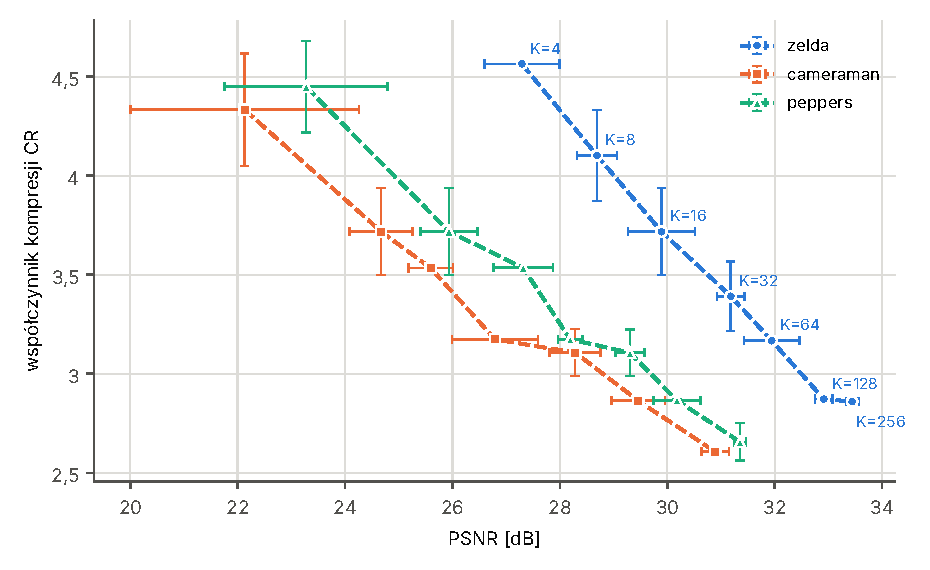
\includegraphics[width=12cm]{fig_cr_psnr.pdf}
 \vspace{-0.3cm}
 \caption{Charakterystyka CR--PSNR dla $K=4,\dots,256$ (kolejne punkty od lewej: rosnące $K$;
 słupki błędów: odchylenie standardowe z~5 uruchomień)}
 \label{fig_crpsnr}
\end{figure}

\noindent Charakterystyka z~Rys.~\ref{fig_crpsnr} pokazuje typowy kompromis kompresji stratnej:
im więcej neuronów, tym lepsza jakość i~tym słabsza kompresja. Dla \texttt{zelda} przejście od
$K=4$ do $K=256$ podnosi PSNR z~$27{,}3$ do $33{,}4$~dB, a~CR spada z~$4{,}56$ do $2{,}86$.
\texttt{cameraman} i~\texttt{peppers} mają przy tych samych $K$ o~2--5~dB niższy PSNR, bo zawierają
więcej ostrych krawędzi i~drobnych szczegółów, których kilka ,,wzorcowych'' ramek nie odtworzy
(Rys.~\ref{fig_odtw}). \texttt{zelda} jest gładsza, a~ramki gładkie są dobrze opisane już przez
sam kierunek ,,płaski'' $[\tfrac12,\tfrac12,\tfrac12,\tfrac12]$ i~jasność.

Przy $K=4$ zwykle przeżywa tylko 1--2 neurony, a~CR jest bliskie ograniczeniu $32/7\approx4{,}57$.
Sieć zapamiętuje wtedy praktycznie tylko jasność ramek, co działa jak zmniejszenie rozdzielczości
obrazu dwukrotnie. Mimo to PSNR wynosi 22--27~dB, bo większość informacji w~obrazie to właśnie
jasność, a~nie ,,tekstura'' wewnątrz ramki $2\times2$.

\begin{figure}[h!]
 \centering
 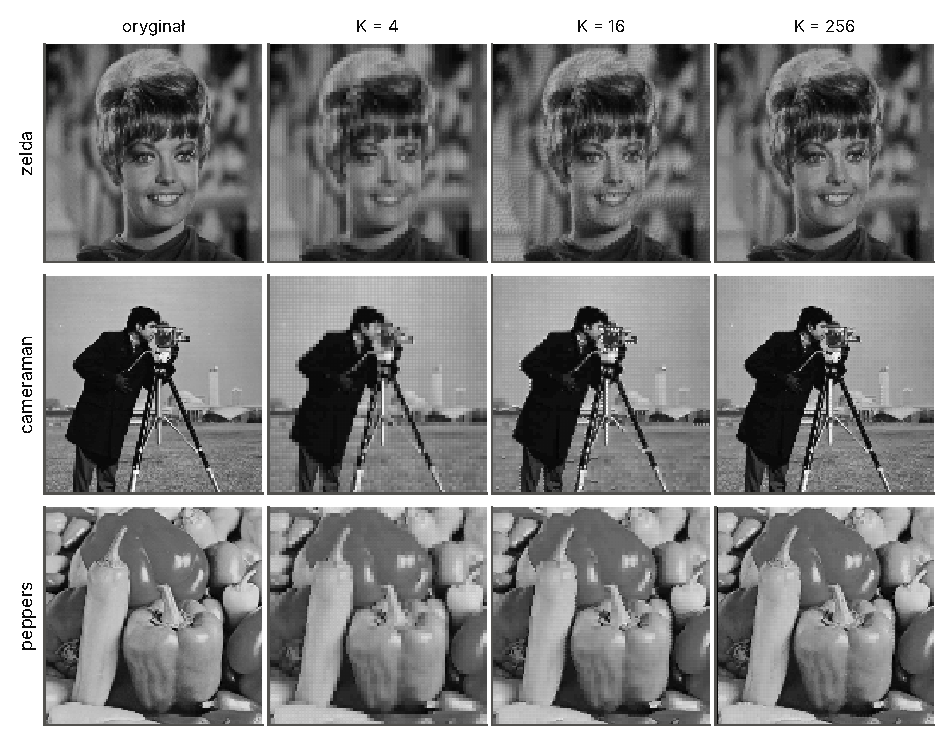
\includegraphics[width=\linewidth]{fig_odtworzone.pdf}
 \vspace{-0.6cm}
 \caption{Obrazy oryginalne i~odtworzone po kompresji dla $K=4$, $16$ i~$256$ (ramka $2\times2$, ziarno 0)}
 \label{fig_odtw}
\end{figure}

\begin{figure}[h!]
 \centering
 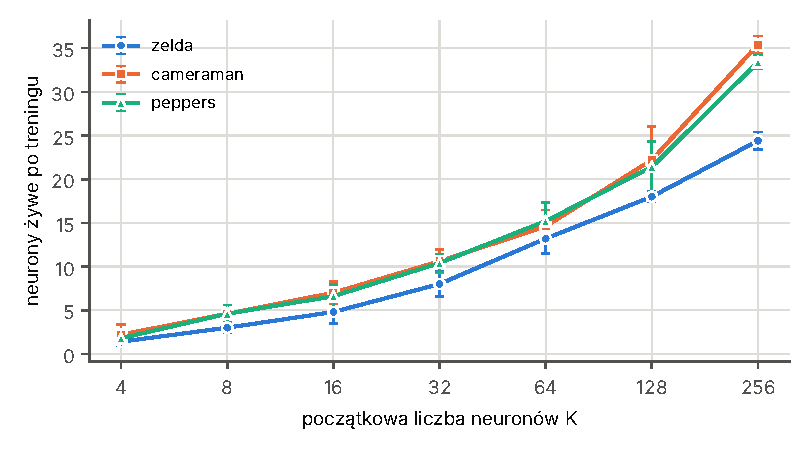
\includegraphics[width=10.5cm]{fig_zywe.pdf}
 \vspace{-0.3cm}
 \caption{Liczba neuronów, które przeżyły trening, w~zależności od początkowej liczby neuronów $K$}
 \label{fig_zywe}
\end{figure}

\textbf{Neurony martwe.} Najważniejsza obserwacja to bardzo duża liczba neuronów martwych
(Tab.~\ref{tab_main}, Rys.~\ref{fig_zywe}). Z~256 neuronów przeżywa tylko 24--35, czyli ok.\ 9--14\%.
Dlatego CR i~PSNR zmieniają się w~funkcji $K$ wolniej, niż wynikałoby z~samej liczby neuronów.
Przy przejściu od 128 do 256 neuronów dla \texttt{zelda} liczba żywych rośnie z~18 do 24, a~indeks
nadal mieści się na 5 bitach, więc CR praktycznie się nie zmienia ($2{,}87\to2{,}86$).

Przyczyna jest geometryczna. Piksele są nieujemne, a~sąsiednie piksele mają zwykle zbliżone wartości,
więc wszystkie znormalizowane ramki leżą w~małym obszarze sfery jednostkowej, blisko kierunku
,,płaskiego'' $\mathbf{u}=[1,\dots,1]/n$. Wagi losowane z~$[-1,1]$ są natomiast rozrzucone po całej
sferze. Neuron wygrywa tylko wtedy, gdy jest bliżej danych niż wszystkie inne neurony, więc
większość neuronów nigdy nie wygrywa (Tab.~\ref{tab_geo}).

\begin{table}[h!]
 \caption{Rozkład kierunków ramek obrazu \texttt{zelda}: kosinus kąta między znormalizowaną ramką
 a~kierunkiem płaskim $\mathbf{u}$ oraz odsetek losowych wektorów z~$[-1,1]^{n^2}$, które trafiają
 w~obszar zajęty przez dane}
 \centering
 \small
 \vspace{0.2cm}
 \begin{tabular}{c c c c c}
  \hline\hline\\[-0.4cm]
  \textbf{Ramka} & \textbf{wymiar} & $\min\cos(\mathbf{x},\mathbf{u})$ & \textbf{mediana} & \textbf{losowe w~obszarze}\\[0.1cm]
  \hline
  $2\times2$ & $4$ & $0{,}680$ & $0{,}998$ & $10{,}49\,\%$ \\
  $4\times4$ & $16$ & $0{,}720$ & $0{,}990$ & $0{,}10\,\%$ \\
  $8\times8$ & $64$ & $0{,}728$ & $0{,}971$ & $0{,}00\,\%$ \\
  \hline
 \end{tabular}
 \label{tab_geo}
\end{table}

\noindent Dla ramki $2\times2$ w~obszar danych trafia ok.\ 10\% losowych wektorów, co zgadza się
z~odsetkiem żywych neuronów. Dla większych ramek ten odsetek spada niemal do zera (eksperyment nr~3).

%%%%%%%%%%%%%%%%%%%%%%%%%%%%%%%%%%%%%%%%%%%%%%%%%%%%%%%%%%%%%%%%%%%%%%%%%%%%%%%%%%%%%%%%%%%%%%%%%%%%%%%%%%%%%%%%%
% PODROZDZIAŁ PT. EKSPERYMENT NR 3
%%%%%%%%%%%%%%%%%%%%%%%%%%%%%%%%%%%%%%%%%%%%%%%%%%%%%%%%%%%%%%%%%%%%%%%%%%%%%%%%%%%%%%%%%%%%%%%%%%%%%%%%%%%%%%%%%

\subsection{Eksperyment nr 3 -- rozmiar ramki i~inicjalizacja wag (dodatkowy)}

\subsubsection{Założenia}

Punkt 5 specyfikacji (opcjonalny). Obraz \texttt{zelda}, ramki $2\times2$, $4\times4$ i~$8\times8$,
$K=4,\dots,256$. Aby sprawdzić, czy słabe wyniki dla dużych ramek wynikają z~neuronów martwych,
porównano też wariant, w~którym wagi początkowe to losowo wybrane (znormalizowane) ramki obrazu
zamiast liczb losowych z~$[-1,1]$. Reszta Algorytmu~2.1 bez zmian.

\subsubsection{Przebieg}

Dla każdego wariantu wykonano 5 treningów i~obliczono średnie CR i~PSNR.

\subsubsection{Rezultat}

\begin{table}[h!]
 \caption{CR / PSNR [dB] dla różnych rozmiarów ramki i~inicjalizacji wag (\texttt{zelda})}
 \centering
 \small
 \vspace{0.2cm}
 \setlength{\tabcolsep}{4pt}
 \begin{tabular}{c c c c c c}
  \hline\hline\\[-0.4cm]
   & \multicolumn{3}{c}{\textbf{wagi losowe z~$[-1,1]$}} & \multicolumn{2}{c}{\textbf{wagi startowe z~obrazu}}\\
  $\boldsymbol{K}$ & $2\times2$ & $4\times4$ & $8\times8$ & $2\times2$ & $4\times4$\\[0.1cm]
  \hline
  16 & $3{,}7$ / $29{,}9$ & $15{,}8$ / $23{,}0$ & $51{,}2$ / $19{,}9$ & $3{,}2$ / $32{,}8$ & $9{,}8$ / $26{,}9$ \\
  64 & $3{,}2$ / $31{,}9$ & $15{,}7$ / $23{,}2$ & $51{,}2$ / $20{,}5$ & $2{,}6$ / $36{,}4$ & $6{,}1$ / $29{,}0$ \\
  256 & $2{,}9$ / $33{,}4$ & $15{,}7$ / $23{,}3$ & $51{,}2$ / $20{,}4$ & $2{,}0$ / $40{,}1$ & $2{,}7$ / $32{,}7$ \\
  \hline
 \end{tabular}
 \label{tab_var}
\end{table}

\begin{figure}[h!]
 \centering
 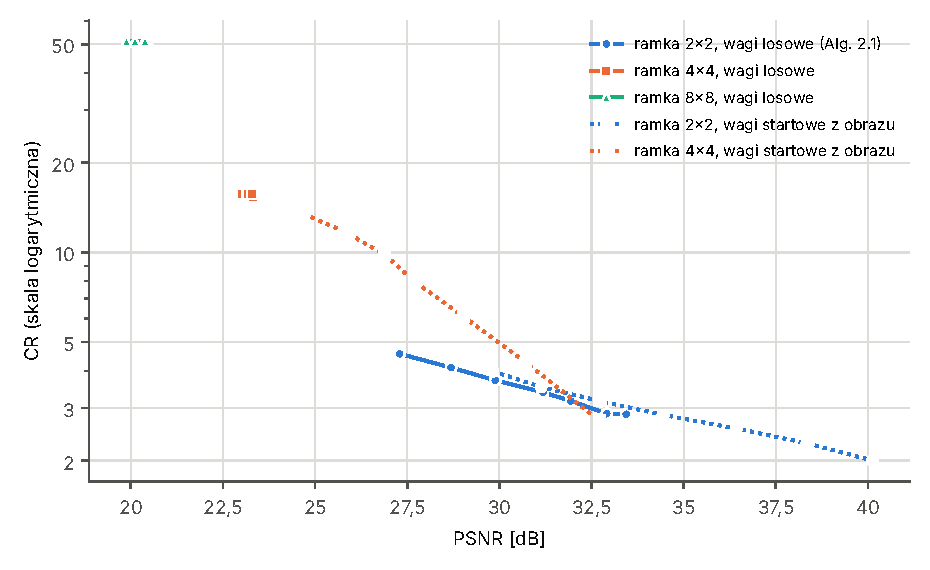
\includegraphics[width=12cm]{fig_warianty.pdf}
 \vspace{-0.3cm}
 \caption{Charakterystyki CR--PSNR dla różnych rozmiarów ramki i~inicjalizacji wag (\texttt{zelda}, $K=4,\dots,256$)}
 \label{fig_war}
\end{figure}

\begin{figure}[h!]
 \centering
 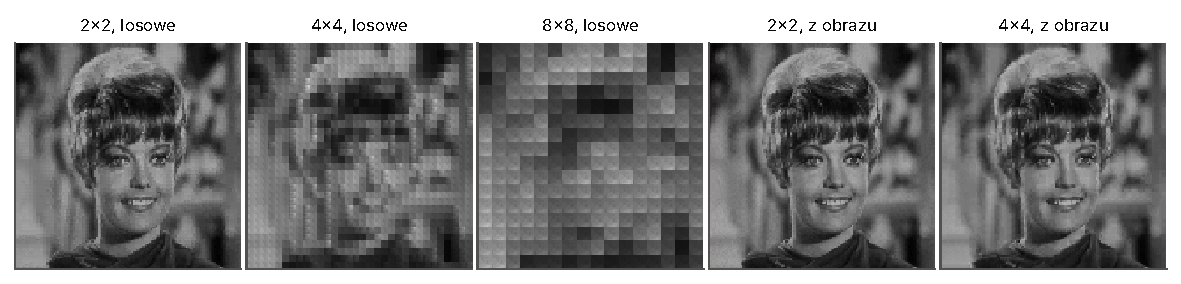
\includegraphics[width=\linewidth]{fig_ramki.pdf}
 \vspace{-0.6cm}
 \caption{Obraz \texttt{zelda} odtworzony dla $K=256$ przy różnych ramkach i~inicjalizacjach}
 \label{fig_ramki}
\end{figure}

\noindent Przy losowej inicjalizacji i~ramkach $4\times4$ oraz $8\times8$ przeżywa niemal zawsze tylko
\textbf{jeden} neuron, niezależnie od $K$. Sieć zapamiętuje wtedy tylko jasność każdej ramki: CR
rośnie do 16 i~51, ale PSNR spada do 23 i~20~dB, a~na obrazie widać wyraźne bloki
(Rys.~\ref{fig_ramki}). Zwiększanie $K$ nic nie daje, bo w~wymiarze 16 czy 64 losowy wektor niemal
nigdy nie trafia w~obszar danych (Tab.~\ref{tab_geo}).

Gdy wagi startowe są ramkami obrazu, wszystkie neurony przeżywają, a~charakterystyka znacznie się
poszerza (Rys.~\ref{fig_war}). Dla ramki $2\times2$ i~$K=256$ PSNR rośnie do $40{,}1$~dB (przy CR $=2{,}0$),
a~ramka $4\times4$ daje płynny zakres od CR $\approx13{,}5$ (PSNR $24{,}7$~dB) do CR $\approx2{,}7$
(PSNR $32{,}7$~dB). Większa ramka pozwala więc osiągnąć wyższe CR, ale pod warunkiem, że neurony
faktycznie się uczą. Przy dużych ramkach i~dużym $K$ rośnie też udział wag w~pliku: dla $8\times8$
i~256 neuronów same wagi zajmowałyby tyle bitów, co cały obraz oryginalny.

\section{Wnioski}

\begin{enumerate}
 \item Zaimplementowana sieć SOM trenowana regułą WTA (Algorytm~2.1) i~schemat kompresji
       z~Algorytmu~2.2 działają poprawnie. Obraz odtworzony z~list $\mathcal{L}$, $\mathcal{T}$,
       $\mathcal{W}$ jest dobrze rozpoznawalny już przy kilku neuronach, a~przy ramce $2\times2$ uzyskano
       CR od ok.\ 2,6 do 4,6 przy PSNR od 22 do 33~dB, zależnie od obrazu i~liczby neuronów.
 \item Liczba neuronów steruje kompromisem jakość--kompresja: więcej neuronów to więcej ,,wzorcowych''
       ramek, wyższy PSNR i~więcej bitów na indeks, czyli niższe CR. Obrazy z~drobnymi szczegółami
       (\texttt{cameraman}, \texttt{peppers}) kompresują się gorzej niż gładki obraz \texttt{zelda}.
 \item Parametry sugerowane w~specyfikacji (20 epok, $\eta=0{,}2$, $q=10$) są rozsądne: PSNR słabo zależy
       od $\eta$ w~zakresie $0{,}05$--$0{,}2$ i~od liczby epok powyżej 5. Współczynnik $q$ to dodatkowe
       pokrętło kompromisu: większe $q$ daje wyższe CR kosztem jakości.
 \item Dla ramki $2\times2$ CR nie może przekroczyć ok.\ $4{,}57$, bo każda ramka wymaga co najmniej
       7 bitów zamiast 32. Wyższe CR wymaga większych ramek.
 \item Głównym ograniczeniem metody są neurony martwe. Ramki obrazu zajmują mały obszar sfery
       jednostkowej, a~wagi losowane z~$[-1,1]$ trafiają tam rzadko: przeżywa ok.\ 10\% neuronów
       dla ramek $2\times2$ i~praktycznie tylko jeden dla ramek $4\times4$ i~$8\times8$. Inicjalizacja
       wag ramkami obrazu usuwa ten problem i~wyraźnie poprawia charakterystykę CR--PSNR.
\end{enumerate}

%%%%%%%%%%%%%%%%%%%%%%%%%%%%%%%%%%%%%%%%%%%%%%%%%%%%%%%%%%%%%%%%%%%%%%%%%%%%%%%%%%%%%%%%%%%%%%%%%%%%%%%%%%%%%%%%%
% PODROZDZIAŁ PT. ZALACZNIKI
%%%%%%%%%%%%%%%%%%%%%%%%%%%%%%%%%%%%%%%%%%%%%%%%%%%%%%%%%%%%%%%%%%%%%%%%%%%%%%%%%%%%%%%%%%%%%%%%%%%%%%%%%%%%%%%%%

\section{Załączniki}

Pełny kod znajduje się w~plikach \texttt{som.py}, \texttt{eksperymenty.py} i~\texttt{wykresy.py}.
Poniżej trening sieci (Algorytm~2.1) i~rdzeń kompresji (Algorytm~2.2) z~pliku \texttt{som.py}:
\begin{lstlisting}[language=Python]
def train(self, X, epochs, eta, rng, shuffle=True):
    X = X[np.linalg.norm(X, axis=1) > 0]
    order = np.arange(len(X))
    for _ in range(epochs):
        if shuffle:
            rng.shuffle(order)
        for k in order:
            x = X[k]
            m = int(np.argmax(self.W @ x))              # neuron zwycieski
            w = self.W[m] + eta * (x - self.W[m])       # w_m = w_m + eta (x - w_m)
            self.W[m] = w / np.linalg.norm(w)           # normalizacja
            self.updated[m] = True

# compress():
frames = image_to_frames(img, frame)                    # ramki n x n -> wektory n^2
Xn, lengths = normalize_rows(frames)
som = SOM(neurons, frame * frame, rng)
som.train(Xn, epochs, eta, rng, shuffle)
K = som.remove_dead()                                   # usuniecie neuronow martwych
L = som.winners(Xn)                                     # lista L - indeksy zwyciezcow
T = np.rint(lengths / q).astype(int)                    # lista T - dlugosci / q
W = quantize_weights(som.W, weight_bits)                # lista W - wagi (8 bitow)
decoded = frames_to_image(q * T[:, None] * W[L], frame, img.shape)
\end{lstlisting}

%%%%%%%%%%%%%%%%%%%%%%%%%%%%%%%%%%%%%%%%%%%%%%%%%%%%%%%%%%%%%%%%%%%%%%%%%%%%%%%%%%%%%%%%%%%%%%%%%%%%%%%%%%%%%%%%%
% BIBLIOGRAFIA
%%%%%%%%%%%%%%%%%%%%%%%%%%%%%%%%%%%%%%%%%%%%%%%%%%%%%%%%%%%%%%%%%%%%%%%%%%%%%%%%%%%%%%%%%%%%%%%%%%%%%%%%%%%%%%%%%

\renewcommand\refname{Bibliografia}
\bibliographystyle{plain}
\bibliography{bibliografia}

\end{document}
